\section{Use Cases} \label{usecases}
\renewcommand{\labelenumii}{\arabic{enumi}.\arabic{enumii}}

We created both the tables for each use case and the complete diagram. Moreover, we created some partial diagrams containing some use cases and organized logically.

\subsection{Tables}
The following are the 42 use case tables.

\subsubsection{Login}
\begin{tabular}{|m{2.5cm}|m{8cm}|}
	\hline
	\multicolumn{2}{|c|}{Login} \\
	\hline
	\textbf{ID} & UC1 - UC\_LOGIN \\
	\hline
	\textbf{Actors} & Registered users (Students, Professors, Publishers, Developers, AI supervisors, Tech Supports, Course Supervisors, System Admins)\\
	\hline
	\textbf{Preconditions} & The user is registered and has credentials \\
	\hline
	\textbf{Sequence} & 
	\begin{enumerate}
		\item The actor selects the login option
		\item The actor inserts its credentials
		\begin{enumerate}
			\item If the actor uses an external authentication system it’s redirected
		\end{enumerate}
		\item Credentials are verified
	\end{enumerate} \\
	\hline
	\textbf{Postconditions} & The user is authenticated and can access its roles’ privileges \\
	\hline
	
	\textbf{Alternative sequence 1} & 
	\begin{enumerate}
		\item The actor inputs the wrong password for the first, second or third time
	\end{enumerate} \\
	\hline
	\textbf{Postconditions} & The user is not authenticated and a notification is sent to the user registered with the inserted username \\
	\hline
	
	\textbf{Alternative sequence 2} & 
	\begin{enumerate}
		\item The actor inputs the wrong password for the fifth time
	\end{enumerate} \\
	\hline
	\textbf{Postconditions} & The user is not allowed to login for a significant time and a notification is sent to the user registered with the inserted username \\
	\hline
	
	\textbf{Alternative sequence 3} & 
	\begin{enumerate}
		\item The actor inputs the wrong username
	\end{enumerate} \\
	\hline
	\textbf{Postconditions} & The user is not authenticated \\
	\hline
\end{tabular}

\subsubsection{Logout}
\begin{tabular}{|m{2.5cm}|m{8cm}|}
	\hline
	\multicolumn{2}{|c|}{Logout} \\
	\hline
	\textbf{ID} & UC2 - UC\_LOGOUT \\
	\hline
	\textbf{Actors} & Registered users (Students, Professors, Publishers, Developers, AI supervisors, Tech Supports, Course Supervisors, System Admins) \\
	\hline
	\textbf{Preconditions} & The user is registered and logged in \\
	\hline
	\textbf{Sequence} & 
	\begin{enumerate}
		\item The actor selects the logout option
		\item The actor confirms their choice
	\end{enumerate} \\
	\hline
	\textbf{Postconditions} & The user is logged out \\
	\hline
\end{tabular}

\subsubsection{Credential recovery}
\begin{tabular}{|m{2.5cm}|m{8cm}|}
	\hline
	\multicolumn{2}{|c|}{Credential recovery} \\
	\hline
	\textbf{ID} & UC3 - UC\_CREDENTIAL\_REC \\
	\hline
	\textbf{Actors} & Registered users (Students, Professors, Publishers, Developers, AI supervisors, Tech Supports, Course Supervisors, System Admins) \\
	\hline
	\textbf{Preconditions} & The user is registered and has forgotten credentials \\
	\hline
	\textbf{Sequence} & 
	\begin{enumerate}
		\item The actor has forgotten their credentials
		\item The actor requires new credentials
	\end{enumerate} \\
	\hline
	\textbf{Postconditions} & The user acquires new credentials on the previously specified recovery channel \\
	\hline
\end{tabular}

\subsubsection{Registration}
\begin{tabular}{|m{2.5cm}|m{8cm}|}
	\hline
	\multicolumn{2}{|c|}{Registration} \\
	\hline
	\textbf{ID} & UC4 - UC\_REGISTRATION \\
	\hline
	\textbf{Actors} & Unregistered users \\
	\hline
	\textbf{Preconditions} & The actor decides to register \\
	\hline
	\textbf{Sequence} & 
	\begin{enumerate}
		\item The actor selects the registration option
		\item The actor decides their credentials, core settings and which roles they want to apply for
		\begin{enumerate}
			\item The credentials’ compliance with security policies is asserted
		\end{enumerate}
	\end{enumerate} \\
	\hline
	\textbf{Postconditions} & The user is registered and has now one or more roles assigned \\
	\hline
	
	\textbf{Alternative sequence 1} & 
	\begin{enumerate}
		\item The actor wants to apply for the Course Supervisor role
		\item The actor provides the apposite proof of identity
	\end{enumerate} \\
	\hline
	\textbf{Postconditions} & The user is registered as a Course Supervisor \\
	\hline
	
	\textbf{Alternative sequence 2} & 
	\begin{enumerate}
		\item The actor inputs incomplete, incorrect or unacceptable credentials/proof
	\end{enumerate} \\
	\hline
	\textbf{Postconditions} & The user is not registered \\
	\hline
\end{tabular}

\subsubsection{Delete Account}
\begin{tabular}{|m{2.5cm}|m{8cm}|}
	\hline
	\multicolumn{2}{|c|}{Delete Account} \\
	\hline
	\textbf{ID} & UC5 - UC\_ACC\_DEL \\
	\hline
	\textbf{Actors} & Registered users (Students, Professors, Publishers, Developers, AI supervisors, Tech Supports, Course Supervisors, System Admins) \\
	\hline
	\textbf{Preconditions} & The user is registered, logged in and decides to delete the account \\
	\hline
	\textbf{Sequence} & 
	\begin{enumerate}
		\item The actor selects the unregistration option
		\item The actor confirms their choice 
		\item The actor confirms their identity by inserting the account’s password
	\end{enumerate} \\
	\hline
	\textbf{Postconditions} & The user is unregistered \\
	\hline
\end{tabular}

\subsubsection{Modify account’s core settings}
\begin{tabular}{|m{2.5cm}|m{8cm}|}
	\hline
	\multicolumn{2}{|c|}{Modify account’s core settings} \\
	\hline
	\textbf{ID} & UC6 - UC\_MOD\_CORE\_SETT \\
	\hline
	\textbf{Actors} & Registered users (Students, Professors, Publishers, Developers, AI supervisors, Tech Supports, Course Supervisors, System Admins) \\
	\hline
	\textbf{Preconditions} & The user is registered, logged in and decides to change one or more of the core settings (e.g. password, username, recovery channel, personal information, …) \\
	\hline
	\textbf{Sequence} & 
	\begin{enumerate}
		\item The actor selects the modify core settings option
		\item The actor confirms their identity by inserting the account’s password
		\item The actor changes the selected settings
		\item The actor confirms the choice
	\end{enumerate} \\
	\hline
	\textbf{Postconditions} & The change in settings is saved \\
	\hline
	
	\textbf{Alternative sequence 1} & 
	\begin{enumerate}
		\item The actor doesn’t confirm their changes or cancels the modification
	\end{enumerate} \\
	\hline
	\textbf{Postconditions} & The settings stay the same \\
	\hline
\end{tabular}

\subsubsection{Modify account’s secondary settings}
\begin{tabular}{|m{2.5cm}|m{8cm}|}
	\hline
	\multicolumn{2}{|c|}{Modify account’s secondary settings} \\
	\hline
	\textbf{ID} & UC7 - UC\_MOD\_SEC\_SETT \\
	\hline
	\textbf{Actors} & Registered users (Students, Professors, Publishers, Developers, AI supervisors, Tech Supports, Course Supervisors, System Admins) \\
	\hline
	\textbf{Preconditions} & The user is registered, logged in and decides to change one or more of the secondary settings (e.g. theme, layout, …) \\
	\hline
	\textbf{Sequence} & 
	\begin{enumerate}
		\item The actor selects the modify secondary settings option
		\item The actor changes the selected settings
		\item The actor confirms the choice
	\end{enumerate} \\
	\hline
	\textbf{Postconditions} & The change in settings is saved \\
	\hline
	
	\textbf{Alternative sequence 1} & 
	\begin{enumerate}
		\item The actor doesn’t confirm their changes or cancels the modification
	\end{enumerate} \\
	\hline
	\textbf{Postconditions} & The settings stay the same \\
	\hline
\end{tabular}

\subsubsection{Modify AI theming}
\begin{tabular}{|m{2.5cm}|m{8cm}|}
	\hline
	\multicolumn{2}{|c|}{Modify AI theming} \\
	\hline
	\textbf{ID} & UC8 - UC\_MOD\_AI\_THEMING \\
	\hline
	\textbf{Actors} & Students, AI supervisors, Tech Supports \\
	\hline
	\textbf{Preconditions} & The user is registered and logged in \\
	\hline
	\textbf{Sequence} & 
	\begin{enumerate}
		\item The user selects the AI theming option
		\item The user inputs a prompt for the AI theming
		\item The user confirms the modification
	\end{enumerate} \\
	\hline
	\textbf{Postconditions} & The theming prompt is modified \\
	\hline
	
	\textbf{Alternative sequence 1} & 
	\begin{enumerate}
		\item The user doesn’t confirm the modification
	\end{enumerate} \\
	\hline
	\textbf{Postconditions} & AI theming continues with the previous prompt \\
	\hline
\end{tabular}

\subsubsection{Access profile and statistics}
\begin{tabular}{|m{2.5cm}|m{8cm}|}
	\hline
	\multicolumn{2}{|c|}{Access profile and statistics} \\
	\hline
	\textbf{ID} & UC9 - UC\_ACCESS\_PROFILE \\
	\hline
	\textbf{Actors} & Registered users (Students, Professors, Publishers, Developers, AI supervisors, Tech Supports, Course Supervisors, System Admins) \\
	\hline
	\textbf{Preconditions} & The user is registered and logged in \\
	\hline
	\textbf{Sequence} & 
	\begin{enumerate}
		\item The actor selects the account display option
	\end{enumerate} \\
	\hline
	\textbf{Postconditions} & The profile with all its statistics is displayed \\
	\hline
\end{tabular}

\subsubsection{Change user role}
\begin{tabular}{|m{2.5cm}|m{8cm}|}
	\hline
	\multicolumn{2}{|c|}{Change user role} \\
	\hline
	\textbf{ID} & UC10 - UC\_USER\_ROLE \\
	\hline
	\textbf{Actors} & Registered users (Students, Professors, Publishers, Developers, AI supervisors, Tech Supports, Course Supervisors, System Admins) \\
	\hline
	\textbf{Preconditions} & The user is registered and logged in \\
	\hline
	\textbf{Sequence} & 
	\begin{enumerate}
		\item The actor selects “User Role” panel
		\item The actor selects the one of the user role from the list
	\end{enumerate} \\
	\hline
	\textbf{Postconditions} & The user role changed following by his dashboard role \\
	\hline
\end{tabular}

\subsubsection{Create course}
\begin{tabular}{|m{2.5cm}|m{8cm}|}
	\hline
	\multicolumn{2}{|c|}{Create course} \\
	\hline
	\textbf{ID} & UC11 - UC\_COURSE\_CREATE \\
	\hline
	\textbf{Actors} & Publishers \\
	\hline
	\textbf{Preconditions} & The user is registered and logged in \\
	\hline
	\textbf{Sequence} & 
	\begin{enumerate}
		\item The actor selects the course panel
		\item The actor selects the “Create new course” option
		\item The actor fills all the mandatory sections for creating a new course
		\item The actor confirms to create new course
	\end{enumerate} \\
	\hline
	\textbf{Postconditions} & The course is created successfully \\
	\hline
	
	\textbf{Alternative sequence 1} & 
	\begin{enumerate}
		\item The actor doesn’t fill all the mandatory sections for creating a new course
		\item The actor confirms to save the unfinished work
	\end{enumerate} \\
	\hline
	\textbf{Postconditions} & The course is saved as draft \\
	\hline
\end{tabular}

\subsubsection{Modify course}
\begin{tabular}{|m{2.5cm}|m{8cm}|}
	\hline
	\multicolumn{2}{|c|}{Modify course} \\
	\hline
	\textbf{ID} & UC12 - UC\_COURSE\_MOD \\
	\hline
	\textbf{Actors} & Professors, Publishers, AI supervisors, Course Supervisors, System Admins \\
	\hline
	\textbf{Preconditions} & The user is registered and logged in \\
	\hline
	\textbf{Sequence} & 
	\begin{enumerate}
		\item The actor selects the course
		\item The actor selects the “Modify course” option
		\item The actor modifies the course
		\item The actor confirms the modification
	\end{enumerate} \\
	\hline
	\textbf{Postconditions} & The course is updated successfully \\
	\hline
	
	\textbf{Alternative sequence 1} & 
	\begin{enumerate}
		\item The actor doesn’t confirm the modification
	\end{enumerate} \\
	\hline
	\textbf{Postconditions} & The course keeps its previous state \\
	\hline
\end{tabular}

\subsubsection{Delete course}
\begin{tabular}{|m{2.5cm}|m{8cm}|}
	\hline
	\multicolumn{2}{|c|}{Delete course} \\
	\hline
	\textbf{ID} & UC13 - UC\_DEL\_COURSE \\
	\hline
	\textbf{Actors} & Publishers, Course Supervisors, System Admins \\
	\hline
	\textbf{Preconditions} & The user is registered and logged in \\
	\hline
	\textbf{Sequence} & 
	\begin{enumerate}
		\item The actor selects “Delete course”
		\item The actor confirms the deletion
	\end{enumerate} \\
	\hline
	\textbf{Postconditions} & The course is deleted \\
	\hline
\end{tabular}

\subsubsection{Archive course}
\begin{tabular}{|m{2.5cm}|m{8cm}|}
	\hline
	\multicolumn{2}{|c|}{Archive course} \\
	\hline
	\textbf{ID} & UC14 - UC\_ARC\_COURSE \\
	\hline
	\textbf{Actors} & Publishers, Course Supervisors, System Admins \\
	\hline
	\textbf{Preconditions} & The user is registered and logged in \\
	\hline
	\textbf{Sequence} & 
	\begin{enumerate}
		\item The actor selects “Archive course”
		\item The actor confirms the modification
	\end{enumerate} \\
	\hline
	\textbf{Postconditions} & The course is moved to archive \\
	\hline
\end{tabular}

\subsubsection{View course}
\begin{tabular}{|m{2.5cm}|m{8cm}|}
	\hline
	\multicolumn{2}{|c|}{View course} \\
	\hline
	\textbf{ID} & UC15 - UC\_COURSE\_VIEW \\
	\hline
	\textbf{Actors} & Registered users (Students, Professors, Publishers, Developers, AI supervisors, Tech Supports, Course Supervisors, System Admins) and Unregistered users \\
	\hline
	\textbf{Preconditions} & The user is registered, logged in and has the right to enter the course \\
	\hline
	\textbf{Sequence} & 
	\begin{enumerate}
		\item The actor select a course from the dashboard or from a library
	\end{enumerate} \\
	\hline
	\textbf{Postconditions} & The course is displayed, along with the global ranking if any minigame is present \\
	\hline
\end{tabular}

\subsubsection{Review course}
\begin{tabular}{|m{2.5cm}|m{8cm}|}
	\hline
	\multicolumn{2}{|c|}{Review course} \\
	\hline
	\textbf{ID} & UC16 - UC\_COURSE\_REV \\
	\hline
	\textbf{Actors} & Registered users (Students, Professors, Publishers, Developers, AI supervisors, Tech Supports, Course Supervisors, System Admins) \\
	\hline
	\textbf{Preconditions} & The user is registered, logged in and has has the right to enter the course. Moreover the course is public and opened\\
	\hline
	\textbf{Sequence} & 
	\begin{enumerate}
		\item The actor leave a review (comment) for the course
	\end{enumerate} \\
	\hline
	\textbf{Postconditions} & The review is added to the course \\
	\hline
\end{tabular}

\subsubsection{Create class}
\begin{tabular}{|m{2.5cm}|m{8cm}|}
	\hline
	\multicolumn{2}{|c|}{Create class} \\
	\hline
	\textbf{ID} & UC17 - UC\_CLASS\_CREATE \\
	\hline
	\textbf{Actors} & Professors \\
	\hline
	\textbf{Preconditions} & The user is registered and logged in \\
	\hline
	\textbf{Sequence} & 
	\begin{enumerate}
		\item The actor selects the class panel
		\item The actor selects the “Create new class” option
		\item The actor fills all the mandatory sections for creating a new class
		\item The actor has possibility to invite Student(s) to the class
		\item The actor confirms to create new class
	\end{enumerate} \\
	\hline
	\textbf{Postconditions} & The class is created successfully \\
	\hline
\end{tabular}

\subsubsection{Modify class}
\begin{tabular}{|m{2.5cm}|m{8cm}|}
	\hline
	\multicolumn{2}{|c|}{Modify class} \\
	\hline
	\textbf{ID} & UC18 - UC\_CLASS\_MOD \\
	\hline
	\textbf{Actors} & Professors, System Admins \\
	\hline
	\textbf{Preconditions} & The user is registered, logged in and has sufficient permissions (owns the class or is admin) \\
	\hline
	\textbf{Sequence} & 
	\begin{enumerate}
		\item The actor selects the class
		\item The actor selects the “Modify class” option
		\item The actor modifies the class
		\item The actor has possibility to invite Student(s) to the class
		\item The actor confirms the modification
	\end{enumerate} \\
	\hline
	\textbf{Postconditions} & The class is updated successfully \\
	\hline
	
	\textbf{Alternative sequence 1} & 
	\begin{enumerate}
		\item The actor doesn’t confirm the modification
	\end{enumerate} \\
	\hline
	\textbf{Postconditions} & The class remains its previous state \\
	\hline
\end{tabular}

\subsubsection{Terminate class}
\begin{tabular}{|m{2.5cm}|m{8cm}|}
	\hline
	\multicolumn{2}{|c|}{Terminate class} \\
	\hline
	\textbf{ID} & UC19 - UC\_CLASS\_TERM \\
	\hline
	\textbf{Actors} & Professors, System Admins \\
	\hline
	\textbf{Preconditions} & The user is registered, logged in and has sufficient permissions (owns the class or is admin) \\
	\hline
	\textbf{Sequence} & 
	\begin{enumerate}
		\item The actor selects “Terminate class”
		\item The actor confirms the termination
	\end{enumerate} \\
	\hline
	\textbf{Postconditions} & The class is terminated, but all the information about the class remains public \\
	\hline
\end{tabular}

\subsubsection{Archive class}
\begin{tabular}{|m{2.5cm}|m{8cm}|}
	\hline
	\multicolumn{2}{|c|}{Archive class} \\
	\hline
	\textbf{ID} & UC20 - UC\_ARC\_CLASS \\
	\hline
	\textbf{Actors} & Professors, System Admins \\
	\hline
	\textbf{Preconditions} & The user is registered, logged in and has sufficient permissions (owns the class or is admin) \\
	\hline
	\textbf{Sequence} & 
	\begin{enumerate}
		\item The actor selects “Archive class”
		\item The actor confirms the modification
	\end{enumerate} \\
	\hline
	\textbf{Postconditions} & The class is moved to archive and all the information about the class is accessible only for Professors and System admins \\
	\hline
\end{tabular}

\subsubsection{View class}
\begin{tabular}{|m{2.5cm}|m{8cm}|}
	\hline
	\multicolumn{2}{|c|}{View class} \\
	\hline
	\textbf{ID} & UC21 - UC\_CLASS\_VIEW \\
	\hline
	\textbf{Actors} & Registered users (Students, Professors, Publishers, Developers, AI supervisors, Tech Supports, Course Supervisors, System Admins) \\
	\hline
	\textbf{Preconditions} & The user is registered and logged in \\
	\hline
	\textbf{Sequence} & 
	\begin{enumerate}
		\item The actor selects a class from the dashboard or from an invitation
	\end{enumerate} \\
	\hline
	\textbf{Postconditions} & The public information of the class is displayed \\
	\hline
\end{tabular}

\subsubsection{Display class’ attendees}
\begin{tabular}{|m{2.5cm}|m{8cm}|}
	\hline
	\multicolumn{2}{|c|}{Display class’ attendees} \\
	\hline
	\textbf{ID} & UC22 - UC\_CLASS\_ATTENDEES \\
	\hline
	\textbf{Actors} & Students, Professors \\
	\hline
	\textbf{Preconditions} & The user is registered, logged in and enrolled in a class \\
	\hline
	\textbf{Sequence} & 
	\begin{enumerate}
		\item The actor selects a class they are enrolled into
	\end{enumerate} \\
	\hline
	\textbf{Postconditions} & The list of people attending the class is displayed \\
	\hline
\end{tabular}

\subsubsection{Display class’ statistics}
\begin{tabular}{|m{2.5cm}|m{8cm}|}
	\hline
	\multicolumn{2}{|c|}{Display class’ statistics} \\
	\hline
	\textbf{ID} & UC23 - UC\_CLASS\_PERFORMANCE \\
	\hline
	\textbf{Actors} & Professors \\
	\hline
	\textbf{Preconditions} & The user is registered, logged in and manages a class \\
	\hline
	\textbf{Sequence} & 
	\begin{enumerate}
		\item The actor selects a class they manage
	\end{enumerate} \\
	\hline
	\textbf{Postconditions} & The performance and statistics of all the attendees is displayed \\
	\hline
\end{tabular}

\subsubsection{Join class}
\begin{tabular}{|m{2.5cm}|m{8cm}|}
	\hline
	\multicolumn{2}{|c|}{Join class} \\
	\hline
	\textbf{ID} & UC24 - UC\_CLASS\_JOIN \\
	\hline
	\textbf{Actors} & Students \\
	\hline
	\textbf{Preconditions} & The user is registered, logged in and has the right to join the class. Moreover the class is opened and public \\
	\hline
	\textbf{Sequence} & 
	\begin{enumerate}
		\item The actor selects “Join class” option
	\end{enumerate} \\
	\hline
	\textbf{Postconditions} & The actor now joined the class. The actor’s information, statistics and progresses for the class is initialized and is public for the class’s owner \\
	\hline
\end{tabular}

\subsubsection{Leave class}
\begin{tabular}{|m{2.5cm}|m{8cm}|}
	\hline
	\multicolumn{2}{|c|}{Leave class} \\
	\hline
	\textbf{ID} & UC25 - UC\_CLASS\_LEAVE \\
	\hline
	\textbf{Actors} & Students \\
	\hline
	\textbf{Preconditions} & The user is registered, logged in and is part of a class\\
	\hline
	\textbf{Sequence} & 
	\begin{enumerate}
		\item The actor selects “Leave class” option
		\item The actor confirm their choice
	\end{enumerate} \\
	\hline
	\textbf{Postconditions} & The actor leaves the class, but their information, statistics and progresses for the class is saved and is still public for the class’s owner \\
	\hline
\end{tabular}

\subsubsection{Publish article}
\begin{tabular}{|m{2.5cm}|m{8cm}|}
	\hline
	\multicolumn{2}{|c|}{Publish article} \\
	\hline
	\textbf{ID} & UC26 - UC\_ART\_PUB \\
	\hline
	\textbf{Actors} & Publisher \\
	\hline
	\textbf{Preconditions} & The user is registered and logged in \\
	\hline
	\textbf{Sequence} & 
	\begin{enumerate}
		\item The actor selects the article panel
		\item The actor selects the “Publish new article” option
		\item The actor fills all the mandatory sections for publishing a new article
		\item The actor confirms to publish new article
	\end{enumerate} \\
	\hline
	\textbf{Postconditions} & The article is published successfully \\
	\hline
\end{tabular}

\subsubsection{Modify article}
\begin{tabular}{|m{2.5cm}|m{8cm}|}
	\hline
	\multicolumn{2}{|c|}{Modify article} \\
	\hline
	\textbf{ID} & UC27 - UC\_ART\_MOD \\
	\hline
	\textbf{Actors} & Publisher, Course Supervisors, System Admins \\
	\hline
	\textbf{Preconditions} & The user is registered and logged in \\
	\hline
	\textbf{Sequence} & 
	\begin{enumerate}
		\item The actor selects the article
		\item The actor selects the “Modify article” option
		\item The actor modifies the article or its visibility
		\item The actor confirms the modification
	\end{enumerate} \\
	\hline
	\textbf{Postconditions} & The article is updated successfully \\
	\hline
	
	\textbf{Alternative sequence 1} & 
	\begin{enumerate}
		\item The actor doesn’t confirm the modification
	\end{enumerate} \\
	\hline
	\textbf{Postconditions} & The article remains in its previous state \\
	\hline
\end{tabular}

\subsubsection{Delete article}
\begin{tabular}{|m{2.5cm}|m{8cm}|}
	\hline
	\multicolumn{2}{|c|}{Delete article} \\
	\hline
	\textbf{ID} & UC28 - UC\_ART\_DEL \\
	\hline
	\textbf{Actors} & Publisher, Course Supervisors, System Admins \\
	\hline
	\textbf{Preconditions} & The user is registered, logged in and has ownership of the article (or is admin) \\
	\hline
	\textbf{Sequence} & 
	\begin{enumerate}
		\item The actor selects “Delete article”
		\item The actor confirms the deletion
	\end{enumerate} \\
	\hline
	\textbf{Postconditions} & The article is deleted \\
	\hline
\end{tabular}

\subsubsection{Archive article}
\begin{tabular}{|m{2.5cm}|m{8cm}|}
	\hline
	\multicolumn{2}{|c|}{Archive article} \\
	\hline
	\textbf{ID} & UC29 - UC\_ART\_ARC \\
	\hline
	\textbf{Actors} & Publisher, Course Supervisors, System Admins \\
	\hline
	\textbf{Preconditions} & The user is registered, logged in and has ownership of the article (or is admin) \\
	\hline
	\textbf{Sequence} & 
	\begin{enumerate}
		\item The actor selects “Archive article”
		\item The actor confirms the modification
	\end{enumerate} \\
	\hline
	\textbf{Postconditions} & The article is moved to archive \\
	\hline
\end{tabular}

\subsubsection{View article}
\begin{tabular}{|m{2.5cm}|m{8cm}|}
	\hline
	\multicolumn{2}{|c|}{View article} \\
	\hline
	\textbf{ID} & UC30 - UC\_ART\_VIEW \\
	\hline
	\textbf{Actors} & Registered users (Students, Professors, Publishers, Developers, AI supervisors, Tech Supports, Course Supervisors, System Admins) and Unregistered users \\
	\hline
	\textbf{Preconditions} & The user is registered and logged in \\
	\hline
	\textbf{Sequence} & 
	\begin{enumerate}
		\item The actor selects an article from the dashboard
	\end{enumerate} \\
	\hline
	\textbf{Postconditions} & The article is opened \\
	\hline
\end{tabular}

\subsubsection{Review article}
\begin{tabular}{|m{2.5cm}|m{8cm}|}
	\hline
	\multicolumn{2}{|c|}{Review article} \\
	\hline
	\textbf{ID} & UC31 - UC\_ART\_REV \\
	\hline
	\textbf{Actors} & Registered users (Students, Professors, Publishers, Developers, AI supervisors, Tech Supports, Course Supervisors, System Admins) \\
	\hline
	\textbf{Preconditions} & The user is registered and logged in. The article is opened and public \\
	\hline
	\textbf{Sequence} & 
	\begin{enumerate}
		\item The actor leave a review (comment) for the article
	\end{enumerate} \\
	\hline
	\textbf{Postconditions} & The review is added to the article \\
	\hline
\end{tabular}

\subsubsection{Create minigame}
\begin{tabular}{|m{2.5cm}|m{8cm}|}
	\hline
	\multicolumn{2}{|c|}{Create minigame} \\
	\hline
	\textbf{ID} & UC32 - UC\_MINIGAME\_CREATE \\
	\hline
	\textbf{Actors} & Developers \\
	\hline
	\textbf{Preconditions} & The user is registered and logged in \\
	\hline
	\textbf{Sequence} & 
	\begin{enumerate}
		\item The actor selects the developer panel
		\item The actor selects the “Create new minigame” option
		\item The actor uses the environment to create the minigame
		\item The actor confirms to create new minigame
	\end{enumerate} \\
	\hline
	\textbf{Postconditions} & The minigame is created successfully and saved to minigame storage \\
	\hline
\end{tabular}

\subsubsection{Modify minigame}
\begin{tabular}{|m{2.5cm}|m{8cm}|}
	\hline
	\multicolumn{2}{|c|}{Modify minigame} \\
	\hline
	\textbf{ID} & UC33 - UC\_MINIGAME\_MOD \\
	\hline
	\textbf{Actors} & Developers, Course Supervisors, System Admin, Tech Supports \\
	\hline
	\textbf{Preconditions} & The user is registered and logged in \\
	\hline
	\textbf{Sequence} & 
	\begin{enumerate}
		\item The actor selects the minigame
		\item The actor selects the “Modify minigame” option
		\item The actor modifies the minigame
		\item The actor confirms the modification
	\end{enumerate} \\
	\hline
	\textbf{Postconditions} & The minigame is updated successfully \\
	\hline
	
	\textbf{Alternative sequence 1} & 
	\begin{enumerate}
		\item The actor doesn’t confirm the modification
	\end{enumerate} \\
	\hline
	\textbf{Postconditions} & The minigame remains in its previous state \\
	\hline
\end{tabular}

\subsubsection{Delete minigame}
\begin{tabular}{|m{2.5cm}|m{8cm}|}
	\hline
	\multicolumn{2}{|c|}{Delete minigame} \\
	\hline
	\textbf{ID} & UC34 - UC\_MINIGAME\_DEL \\
	\hline
	\textbf{Actors} & Developers, Course Supervisors, System Admin \\
	\hline
	\textbf{Preconditions} & The user is registered, logged in and owns the minigame (or is admin) \\
	\hline
	\textbf{Sequence} & 
	\begin{enumerate}
		\item The actor selects “Delete minigame”
		\item The actor confirms the deletion
	\end{enumerate} \\
	\hline
	\textbf{Postconditions} & The minigame is deleted from memory and from all the courses containing it \\
	\hline
\end{tabular}

\subsubsection{Archive minigame}
\begin{tabular}{|m{2.5cm}|m{8cm}|}
	\hline
	\multicolumn{2}{|c|}{Archive minigame} \\
	\hline
	\textbf{ID} & UC35 - UC\_MINIGAME\_ARC \\
	\hline
	\textbf{Actors} & Developers, Course Supervisors, System Admin \\
	\hline
	\textbf{Preconditions} & The user is registered, logged in and owns the minigame (or is admin) \\
	\hline
	\textbf{Sequence} & 
	\begin{enumerate}
		\item The actor selects “Archive minigame”
		\item The actor confirms the modification
	\end{enumerate} \\
	\hline
	\textbf{Postconditions} & The minigame is moved to archive and is deleted from all the courses containing it \\
	\hline
\end{tabular}

\subsubsection{Register minigame from developer}
\begin{tabular}{|m{2.5cm}|m{8cm}|}
	\hline
	\multicolumn{2}{|c|}{Register minigame from developer} \\
	\hline
	\textbf{ID} & UC36 - UC\_MINIGAME\_REG\_DEV \\
	\hline
	\textbf{Actors} & Developers \\
	\hline
	\textbf{Preconditions} & The user is registered and logged in \\
	\hline
	\textbf{Sequence} & 
	\begin{enumerate}
		\item The actor selects the minigame
		\item The actor selects “Register minigame to course”
		\item The actor chooses the course(s) to register (add) minigame into
		\item The actor fills all the mandatory sections for registering a new minigame to course
		\item The actor confirms to register minigame
	\end{enumerate} \\
	\hline
	\textbf{Postconditions} & The minigame is register successfully to the course(s) \\
	\hline
\end{tabular}

\subsubsection{Register minigame from observer}
\begin{tabular}{|m{2.5cm}|m{8cm}|}
	\hline
	\multicolumn{2}{|c|}{Register minigame from observer} \\
	\hline
	\textbf{ID} & UC37 - UC\_MINIGAME\_REG \\
	\hline
	\textbf{Actors} & Publishers, Developers, AI supervisors, Tech Supports, Course Supervisors, System Admins \\
	\hline
	\textbf{Preconditions} & The user is registered, logged in and has authorization from minigame owner \\
	\hline
	\textbf{Sequence} & 
	\begin{enumerate}
		\item The actor selects the course
		\item The actor selects the “Modify course” option
		\item The actor selects “Register minigame to course”
		\item The actor chooses the minigame to add to course
		\item The actor fills all the mandatory sections for registering a new minigame to course
		\item The actor confirms to register minigame
	\end{enumerate} \\
	\hline
	\textbf{Postconditions} & The minigame is register successfully to the course(s) \\
	\hline
\end{tabular}

\subsubsection{Play minigame}
\begin{tabular}{|m{2.5cm}|m{8cm}|}
	\hline
	\multicolumn{2}{|c|}{Delete course} \\
	\hline
	\textbf{ID} & UC38 - UC\_PLAY \\
	\hline
	\textbf{Actors} & Registered users (Students, Professors, Publishers, Developers, AI supervisors, Tech Supports, Course Supervisors, System Admins) and Unregistered users \\
	\hline
	\textbf{Preconditions} & The user opens the minigame \\
	\hline
	\textbf{Sequence} & 
	\begin{enumerate}
		\item The actor plays the minigame
	\end{enumerate} \\
	\hline
	\textbf{Postconditions} & The actor can play the minigame \\
	\hline
\end{tabular}

\subsubsection{Pay developer}
\begin{tabular}{|m{2.5cm}|m{8cm}|}
	\hline
	\multicolumn{2}{|c|}{Pay developer} \\
	\hline
	\textbf{ID} & UC39 - UC\_PAY \\
	\hline
	\textbf{Actors} & Publishers \\
	\hline
	\textbf{Preconditions} & The user is registered, logged in and has tasked a developer with a minigame \\
	\hline
	\textbf{Sequence} & 
	\begin{enumerate}
		\item The actor selects the payment option
		\item The user selects the external payment method they want to use
		\item The actor follows the external payment system iter
	\end{enumerate} \\
	\hline
	\textbf{Postconditions} & The actor has paid the developer \\
	\hline
\end{tabular}

\subsubsection{Use tech support chat}
\begin{tabular}{|m{2.5cm}|m{8cm}|}
	\hline
	\multicolumn{2}{|c|}{Use tech support chat} \\
	\hline
	\textbf{ID} & UC40 - UC\_SUPPORT\_CHAT \\
	\hline
	\textbf{Actors} & Registered users (Students, Professors, Publishers, Developers, AI supervisors, Tech Supports, Course Supervisors, System Admins) \\
	\hline
	\textbf{Preconditions} & The user is registered, logged in and has a technical problem \\
	\hline
	\textbf{Sequence} & 
	\begin{enumerate}
		\item The actor opens the tech support chat
		\item The user sends/receives a message on the chat
	\end{enumerate} \\
	\hline
	\textbf{Postconditions} & The actor interacts with Tech Supports and starts solving the technical problem \\
	\hline
\end{tabular}

\subsubsection{Use development chat}
\begin{tabular}{|m{2.5cm}|m{8cm}|}
	\hline
	\multicolumn{2}{|c|}{Use development chat} \\
	\hline
	\textbf{ID} & UC41 - UC\_DEV\_CHAT \\
	\hline
	\textbf{Actors} & Publishers, Developers \\
	\hline
	\textbf{Preconditions} & The user is registered, logged in and has the need to discuss about minigame creation \\
	\hline
	\textbf{Sequence} & 
	\begin{enumerate}
		\item The actor opens the development chat
		\item The actor communicates with the commissioner/developer
	\end{enumerate} \\
	\hline
	\textbf{Postconditions} & The actor interacts with Developer/commissioner and starts the minigame development process \\
	\hline
\end{tabular}

\subsubsection{Search element}
\begin{tabular}{|m{2.5cm}|m{8cm}|}
	\hline
	\multicolumn{2}{|c|}{Search element} \\
	\hline
	\textbf{ID} & UC42 - UC\_SEARCH \\
	\hline
	\textbf{Actors} & Registered users (Students, Professors, Publishers, Developers, AI supervisors, Tech Supports, Course Supervisors, System Admins) and Unregistered users \\
	\hline
	\textbf{Preconditions} & The user wants to find some material on the platform (course, class, mini-game, article, …) \\
	\hline
	\textbf{Sequence} & 
	\begin{enumerate}
		\item The actor selects the search option
		\item The actor inputs the possible search parameters (name, subject, type, …)
	\end{enumerate} \\
	\hline
	\textbf{Postconditions} & A list of resources adhering to the parameters is displayed \\
	\hline
\end{tabular}

\subsubsection{Remove review}
\begin{tabular}{|m{2.5cm}|m{8cm}|}
	\hline
	\multicolumn{2}{|c|}{Remove review} \\
	\hline
	\textbf{ID} & UC43 - UC\_DEL\_REV \\
	\hline
	\textbf{Actors} & System Admins \\
	\hline
	\textbf{Preconditions} & The user is registered and logged in. The chosen review violates some policies of the platform \\
	\hline
	\textbf{Sequence} & 
	\begin{enumerate}
		\item The actor removes review from any material
	\end{enumerate} \\
	\hline
	\textbf{Postconditions} & The review is removed entirely \\
	\hline
\end{tabular}

\newpage
\subsection{Diagrams}
\begin{figure}[h]
	\centering
	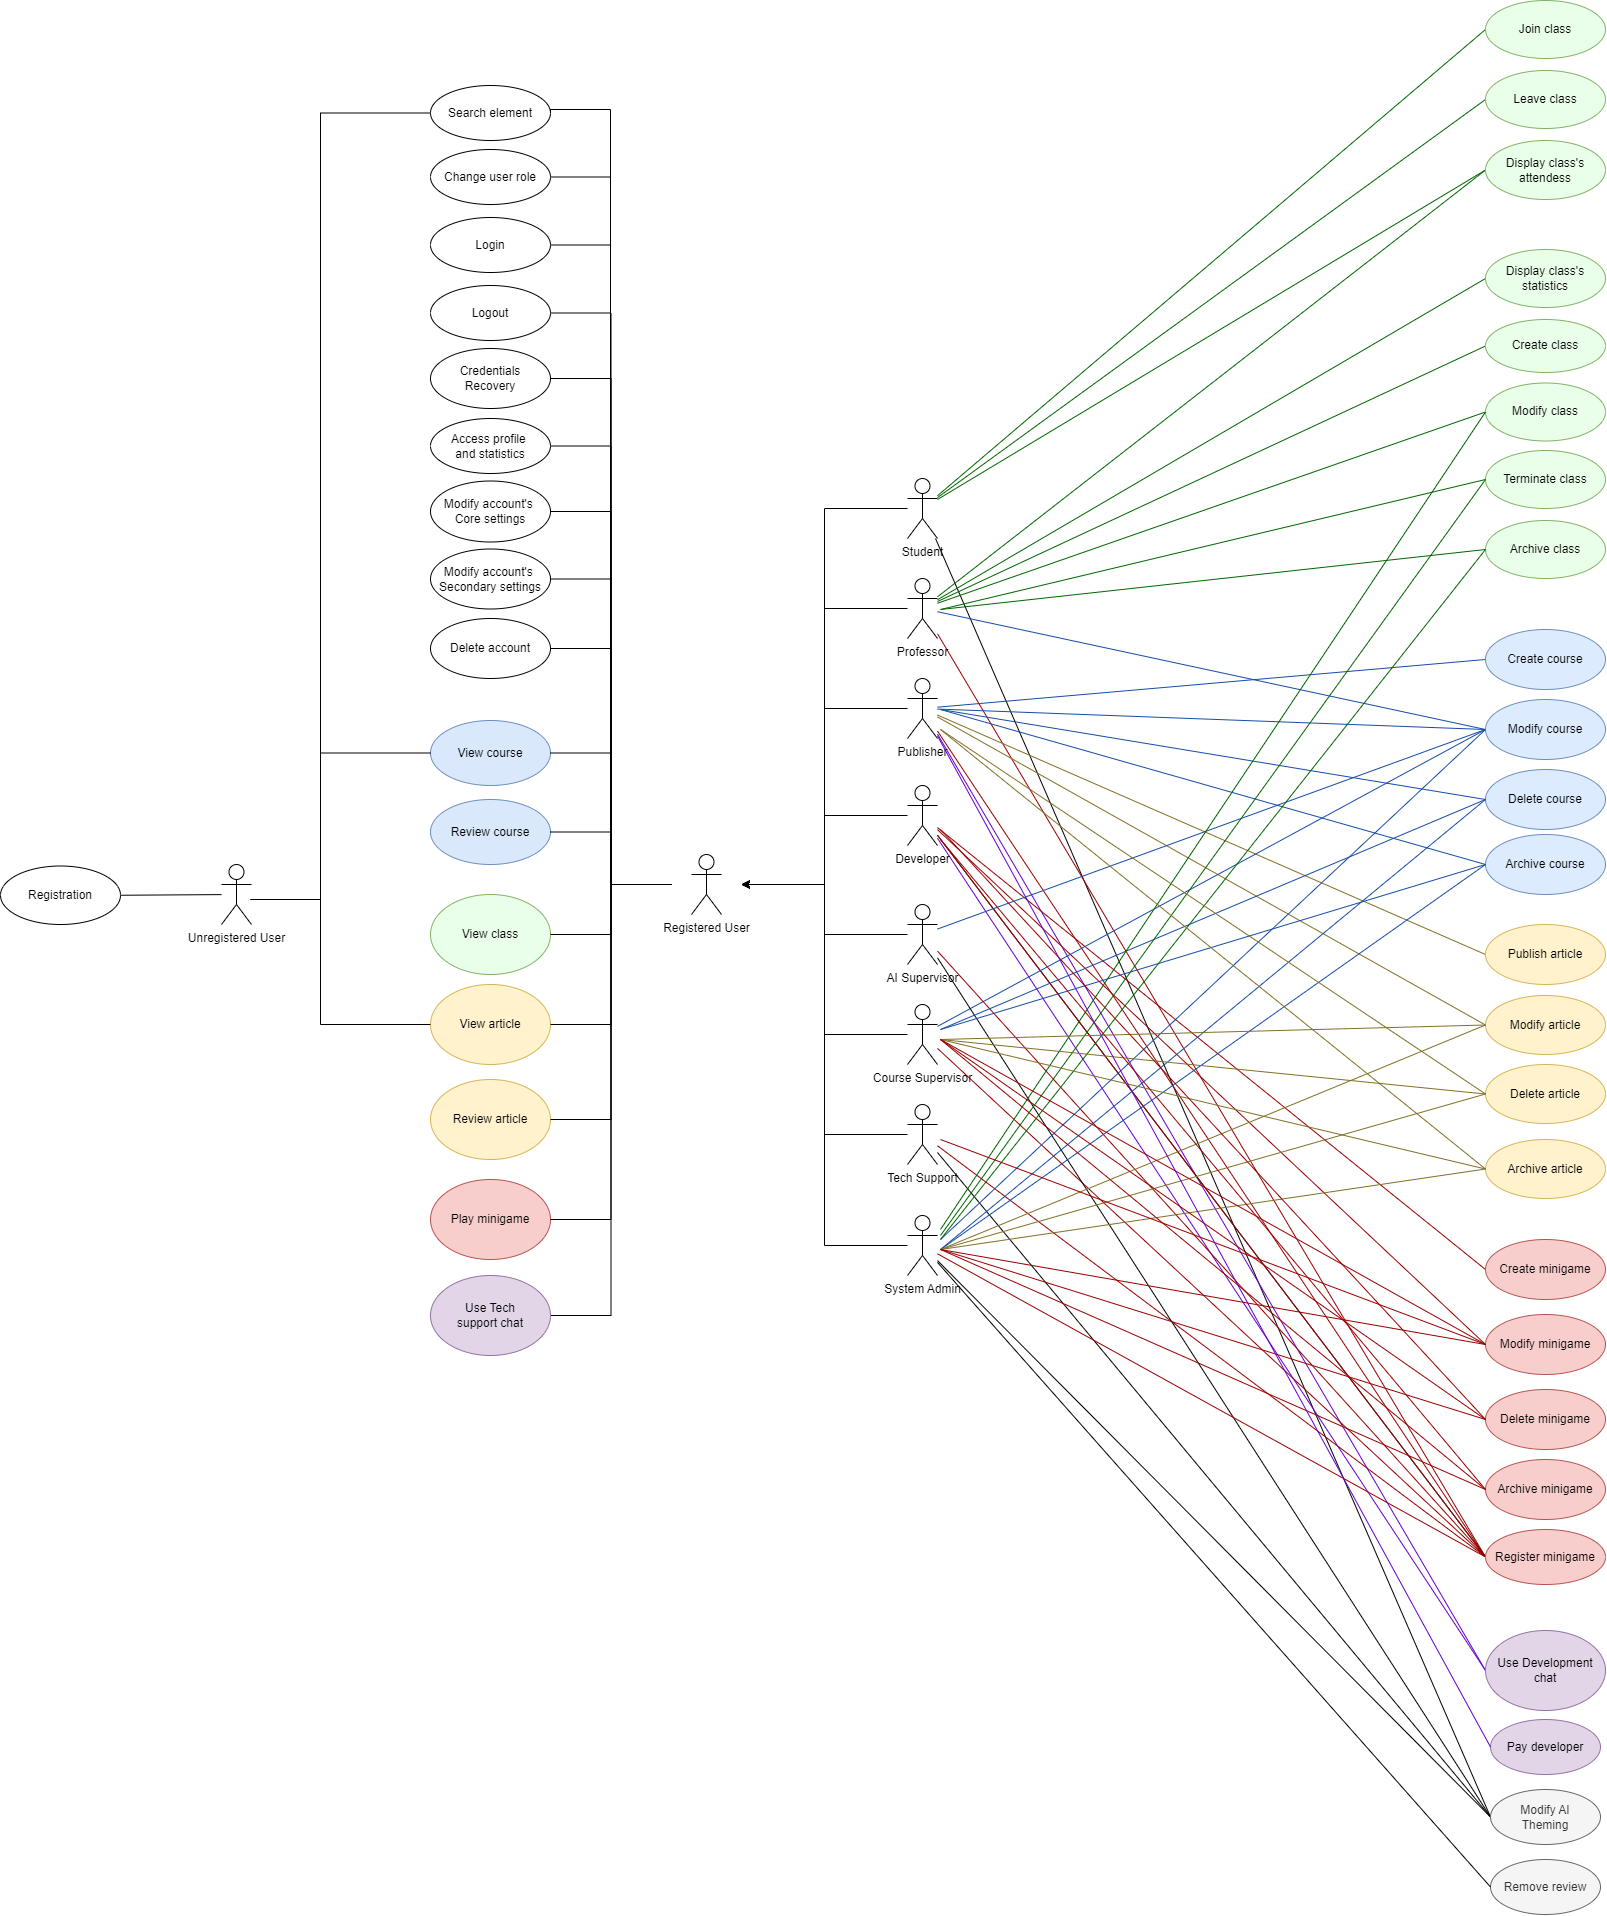
\includegraphics[width=0.9\textwidth]{images/usecase-diagram.png}
	\caption{Complete use case diagram}
	\label{fig:usecase-diagram}
\end{figure}

\newpage
\subsubsection{Account and general purpose}
\begin{figure}[h]
	\centering
	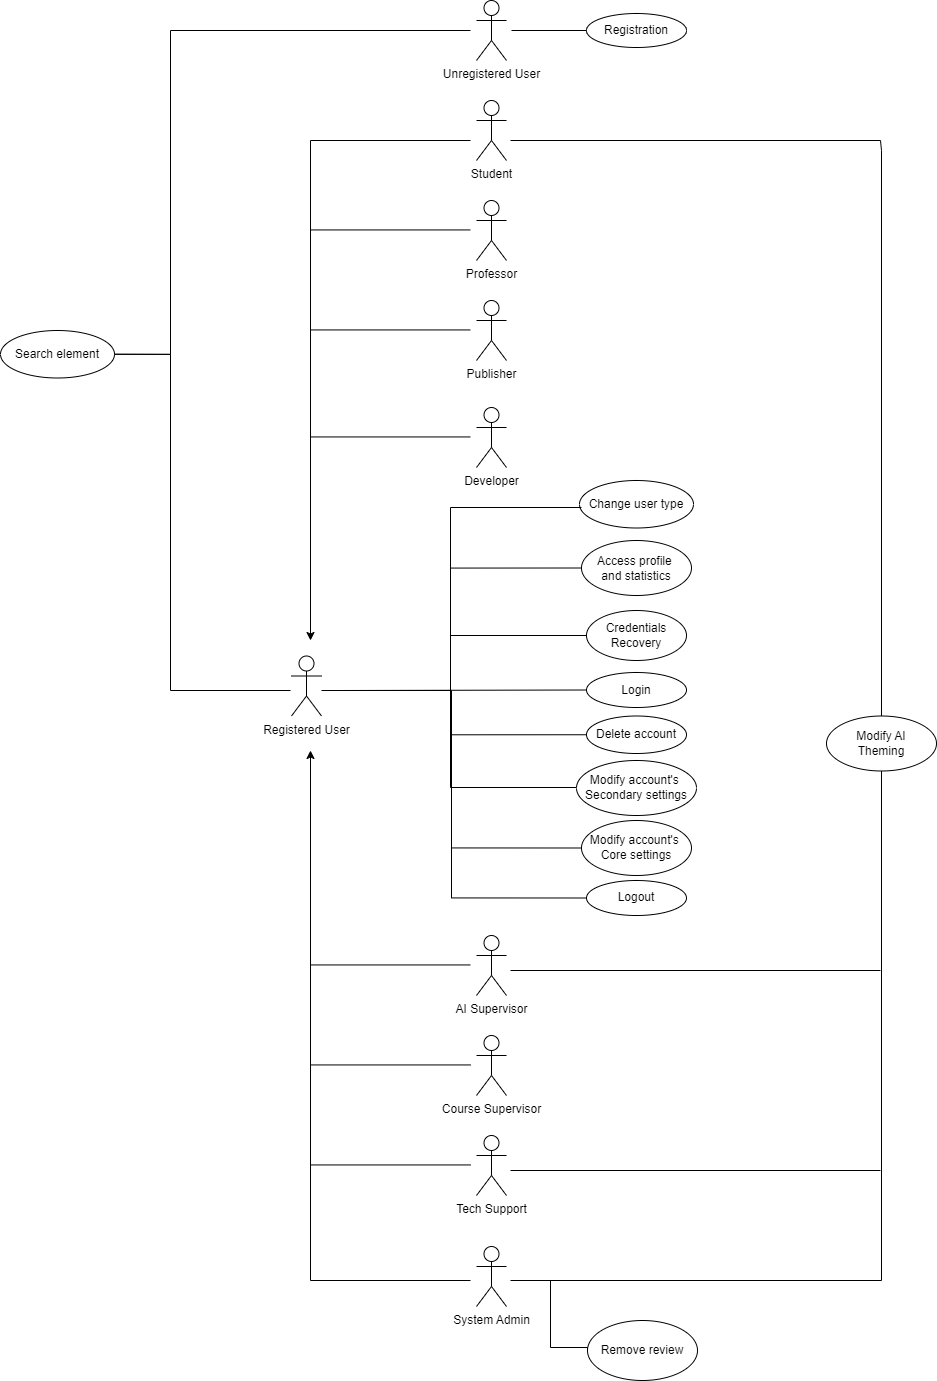
\includegraphics[width=0.7\textwidth]{images/UC-account.png}
	\caption{Use case diagram for account system}
	\label{fig:UC-account}
\end{figure}

\newpage
\subsubsection{Article}
\begin{figure}[h]
	\centering
	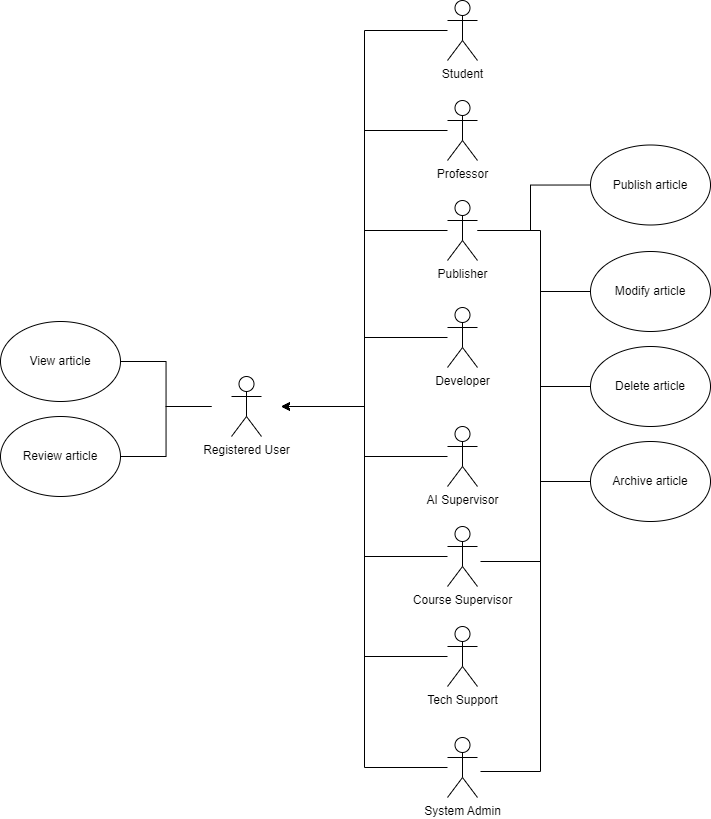
\includegraphics[width=0.9\textwidth]{images/UC-article.png}
	\caption{Use case diagram for article system}
	\label{fig:UC-article}
\end{figure}

\newpage
\subsubsection{Chat}
\begin{figure}[h]
	\centering
	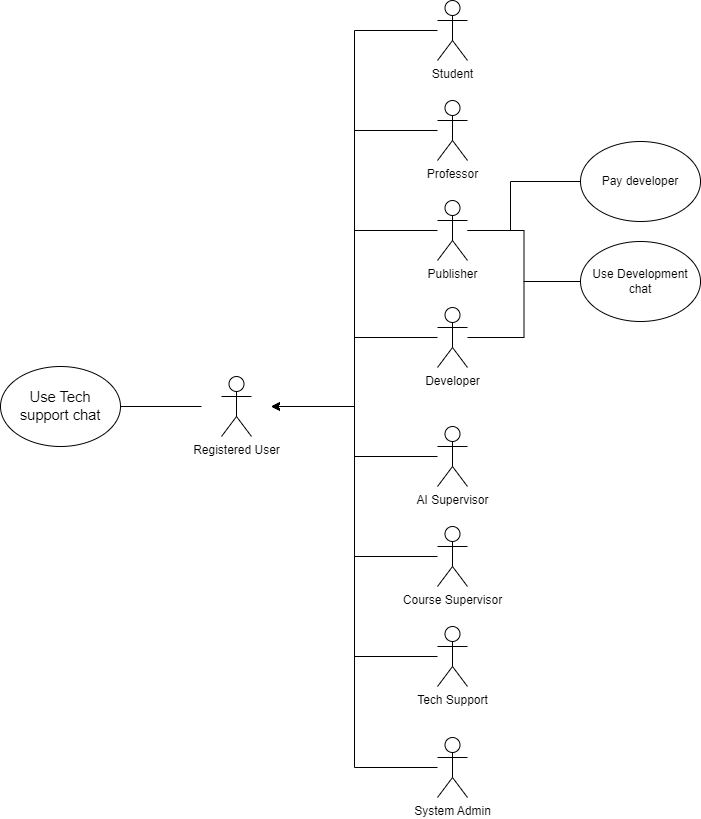
\includegraphics[width=0.9\textwidth]{images/UC-chat.png}
	\caption{Use case diagram for chat system}
	\label{fig:UC-chat}
\end{figure}

\newpage
\subsubsection{Class}
\begin{figure}[h]
	\centering
	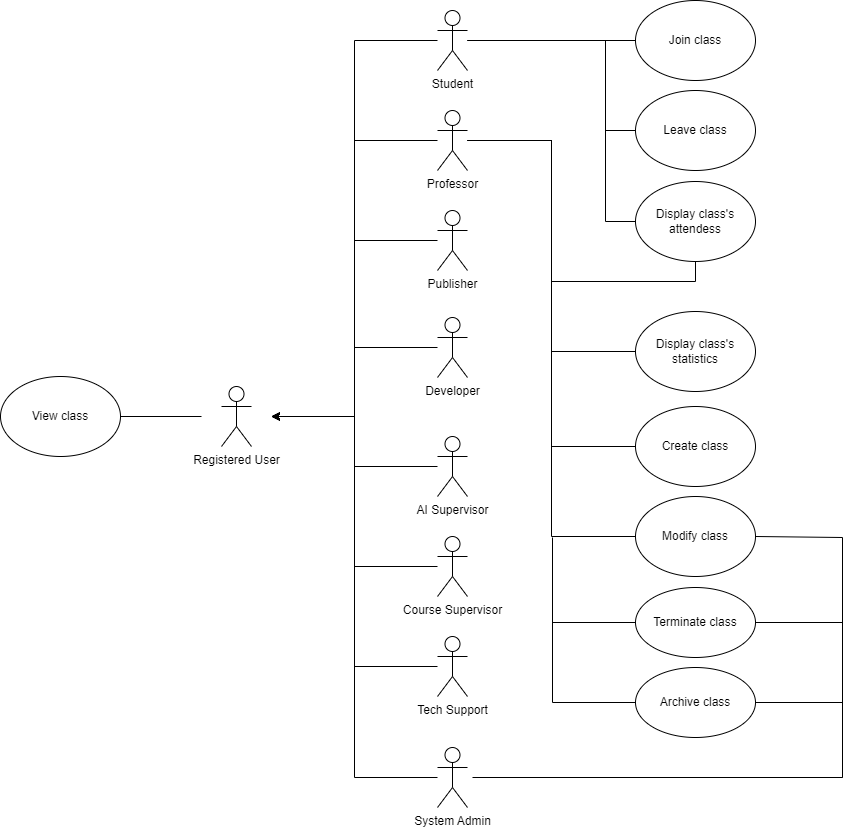
\includegraphics[width=0.9\textwidth]{images/UC-class.png}
	\caption{Use case diagram for class system}
	\label{fig:UC-class}
\end{figure}

\newpage
\subsubsection{Course}
\begin{figure}[h]
	\centering
	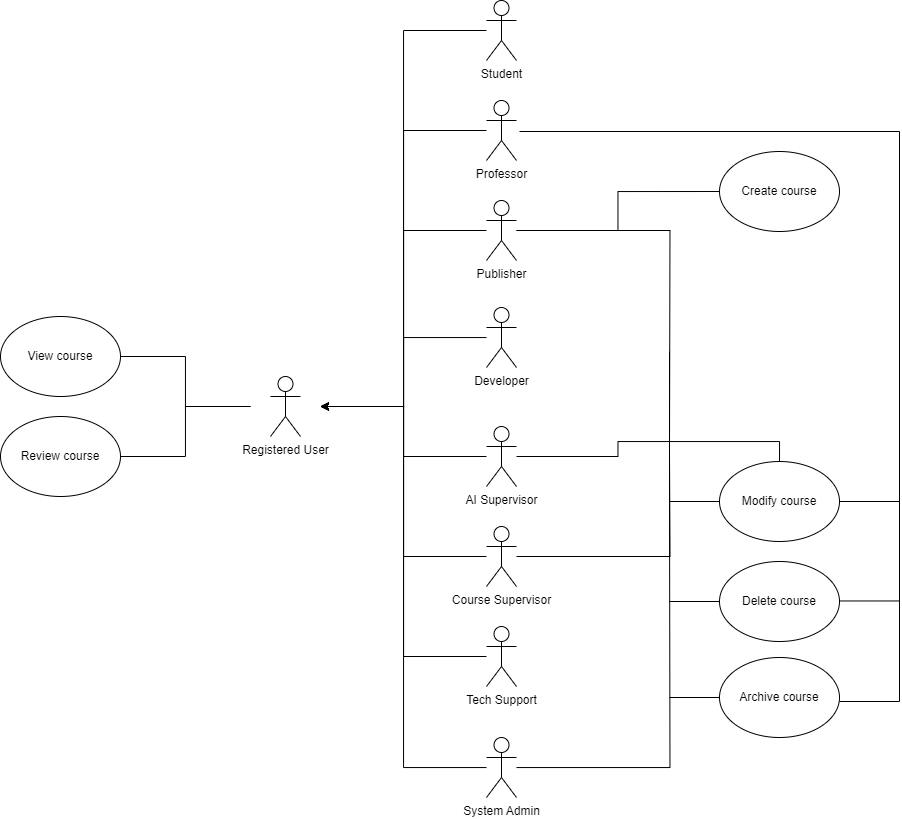
\includegraphics[width=0.9\textwidth]{images/UC-course.png}
	\caption{Use case diagram for course system}
	\label{fig:UC-course}
\end{figure}

\newpage
\subsubsection{Minigame}
\begin{figure}[h]
	\centering
	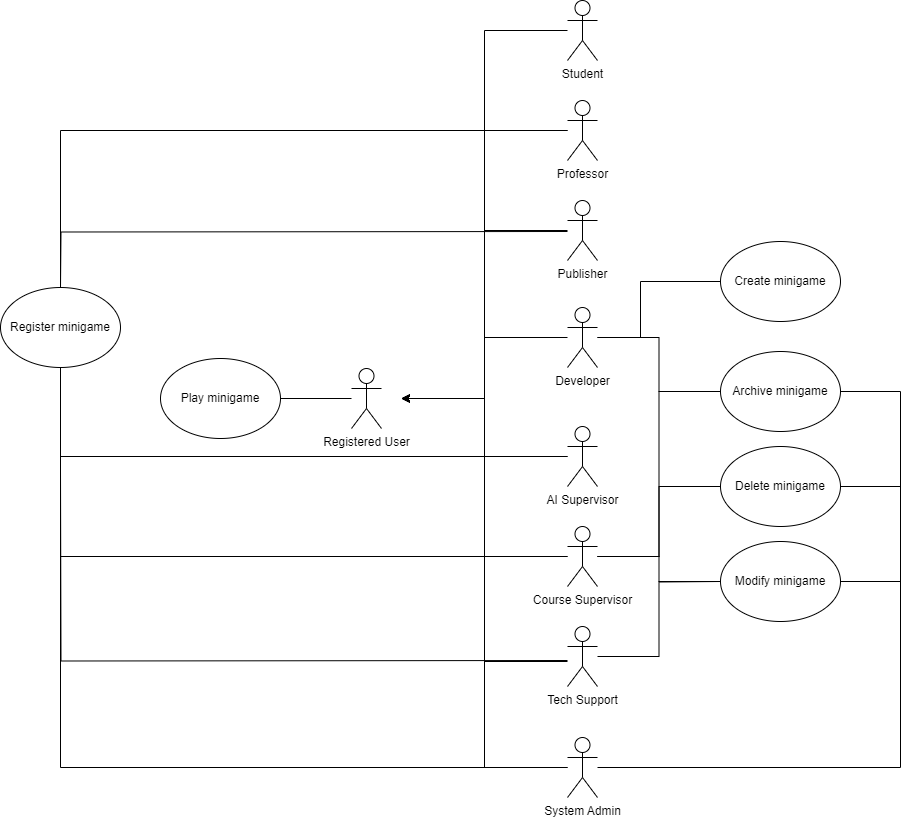
\includegraphics[width=0.9\textwidth]{images/UC-minigame.png}
	\caption{Use case diagram for minigame system}
	\label{fig:UC-course}
\end{figure}
